\documentclass[a4paper,10pt]{article}
%\usepackage[utf8x]{inputenc}
\usepackage{amsmath}
\usepackage{graphicx}
%opening
\title{Programming Techniques for Scientific Simulations: Report 1}
\author{Marion Baumgartner}

\begin{document}

\maketitle

\section{Description of the Tasks with Results}
\subsection{Endianness}
The endianness basically tells us how the bytes are ordered. We say that a machine has little endianness if the least significant byte is first. If the most significant byte is first then the machine has big endianness. If we take for example a 32 bit integer which is stored in 4 bytes we get \\
Byte 3; Byte 2; Byte 1; Byte 0\\


In a little endian we have the following arrangement:\\
BaseAddress+0 Byte0\\
BaseAddress+1 Byte1\\
BaseAddress+2 Byte2\\
BaseAddress+3 Byte3.


For a big endian we get\\
BaseAddress+0 Byte3\\
BaseAddress+1 Byte2\\
BaseAddress+2 Byte1\\
BaseAddress+3 Byte0.


In order to check weather a machine has little or big endianness we can simply check how it sores an n-bit integer (this takes n/8 bytes)

The result for my computer is that it has little endian :).

\subsection{Machine Epsilon}
The machine $\epsilon$ is the smallest number such that $1+\epsilon \neq 1$.


What the program does is it take an initial $\epsilon=1$ and then check if $1+\epsilon \neq 1$ if this is true then we decrease $epsilon$ by $\frac{1}{2}$ and check again. This is repeated until we find an $\epsilon$ which does not fulfil the criteria. At this point we know that the $\epsilon$ we had one step before is what we are looking for. This can be done for float, double and long double. The main idea is always the same, just the data types change.

On my computer I get that the precision for
\begin{itemize}
	\item float $=2.22045e-16$
	\item double $= 2.22045e-16$
	\item long double $= 1.0842e-19$
\end{itemize}	

Now the problem was revised using templates. Before I programmed it a bit ugly and due to the fact that i did not inline the epsilon function it made the program rather 

Now the new results which I got are

\begin{itemize}	
	\item Float epsilon $= 1.0842e-19$
	\item Double epsilon $= 1.0842e-19$
	\item Int epsilon $= 1$
	\item Unsigned int epsilon $= 1$
\end{itemize}

Now I am getting the that the machine epsilon for a Float and a double is the same as I originally got for a long double. This is actually because may program had a bug which I did not realize at the beginning. To fix the bug the a cast has to be made to force the compiler to use the correct type.

\subsection{Cache Effects}[h!]
\begin{figure}
\centering
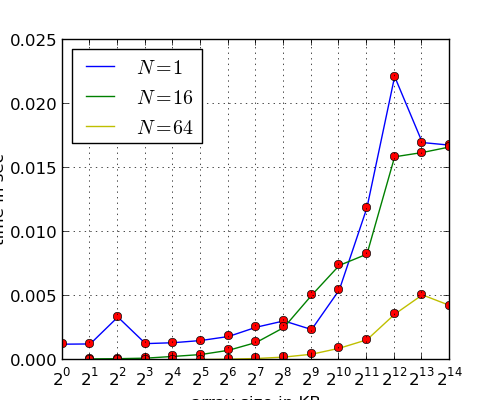
\includegraphics[scale=0.8]{CacheSize.png} 
\caption{The image shows the array size on the x-axis (the scale shows $2^{X \text{MB}}$) and the time in seconds on the y-axis (sorry the axes naming was cut off)}
\label{fig1}
\end{figure}

The aim of this exercise was to determine the cache size of the computer. If I look up the the CPU information on my PC I get that I have 2 processors each with a cache size of about $6$MB. I found this using "cat /proc/cpuinfocat /proc/cpuinfo"

An other way to see this is by using a c++ program (For close description see Exercise 6 and  task1b.cpp).

The result which I got is plotted in figure \ref{fig1}
%% include Figure 

The figure shows the array size v.s the access time it takes to access $N$ elements in the array. Of course if we access fewer elements the access time is reduced. Now looking at the figure we can see that the time says about the same up until the array has a size of about $2^6$B $\sim 6$KB. Then the slops again gets steeper at about $2^12$ where we are at about $12$M.
As we look at the three different curves on the figure we see they follow about the same rule. From this we can guess that the first and the second cache size is at about $6$MB. 


A further observation we can make in the figure is that the line where $N=1$ raises very quickly between $10$MB and $12$MB. Then al of a sudden it falls again. This can be explained by the fact that CPUs nowadays accesses memories in big blocks (cache lines).This means that when a particular memory location is read, the entire cache line is fetched from the main memory into the cache.  Then Accessing other values from the same cache line is cheap. (This is something I learned, and as well that this is important for efficient programming.)

\end{document}
